\documentclass[11pt]{report}
\clubpenalty=10000
\widowpenalty=10000

% It is handy to define new commands for text that occurs frequently (see Discussion)
\newcommand{\MT}{^{\mathrm{MT}}}
\newcommand{\ga}{\gtrsim}
\newcommand{\Lpot}{(L+1)^2}
\newcommand{\WS}{^{\mathrm{WS}}}
\newcommand{\fracd}[2]{\frac{\displaystyle{#1}}{\displaystyle{#2}}} 

%--Format the section headers

%\usepackage{nameref}
\usepackage{amsmath}
\usepackage{amsfonts}
\usepackage{amssymb}
\usepackage{wasysym}
\usepackage{graphicx}
\usepackage{pslatex}
\usepackage{lscape}
\usepackage[T1]{fontenc}
\usepackage[latin1]{inputenc}
\usepackage{longtable}
 \setlength{\LTcapwidth}{5.5 in}
\usepackage{chapterbib}
\usepackage{fancyhdr} % for better header layout
\usepackage{eucal}
\usepackage[english]{babel}
\usepackage[usenames, dvipsnames]{color}
\usepackage[perpage]{footmisc}
\usepackage[round, sort, numbers, authoryear]{natbib}
%\usepackage{multicol} % for pages with multiple text columns, e.g. References
\setlength{\columnsep}{20pt} % space between columns; default 10pt quite narrow
\usepackage[nottoc]{tocbibind} % correct page numbers for bib in TOC, nottoc suppresses an entry for TOC itself
\usepackage{geometry}
\usepackage{setspace}
\usepackage{url}
\usepackage{lastpage}

% FJS Changed this... I didn't like the numbering or the
% indentation... so I introduced a fake chapter Main Text. 
\setcounter{secnumdepth}{0}
\setcounter{tocdepth}{5}

%--set the page formatting--
\geometry{hmargin={1.6in,1.1in},vmargin={1.5in,1.2in}}
\doublespacing

\begin{document}
%--front matter needs roman pagination--
\pagenumbering{roman}

%--Title Page--
\thispagestyle{empty}
  \begin{center}
    \textsc{\LARGE Using Princeton Precipitation climatology to predict future precipitation events} %Fill in your information
  \end{center}
  \vspace{.6in}
  \begin{center}
      Tyrone Zhang
  \end{center}
  \vspace{.6in}
  \begin{center}
    \textsc{A Senior Thesis \\ %Fill in your information
    Presented to the Faculty \\
    of Princeton University \\
    in Candidacy for the Degree \\
    of Bachelor of Arts}
  \end{center}
  \vspace{.3in}
  \begin{center}
    \textsc{Recommended for Acceptance \\
    by the \\Department of  Geosciences \\}
    Adviser: Frederik J.~Simons
  \end{center}
  \vspace{.3in}
  \begin{center}
  \today
  \end{center}
  
  \clearpage


%--Copyright Page--
\thispagestyle{empty}
\vspace*{3in}
\begin{center}
\emph{This paper represents my own work in accordance with University regulations,} \\
Tyrone Zhang %%Sign here
\end{center}
\clearpage

%--Abstract--  
\addcontentsline{toc}{chapter}{Abstract}
\begin{center}
\Large \textbf{Abstract}
\end{center}
 
% Senior thesis or Junior Project Abstract -----------------------------------------------------

%Delete the text below and write your abstract
Princeton's climate is one that has four seasons and a high temperature variation through the year. The precipitation in Princeton is spread out throughout the year. Precipitation events are often characterized by an exponential distribution of both the duration and the total precipitation per event. The shortest precipitation events and the smallest precipitation totals are the most frequent, while the longer the precipitation event, the less likely it is to occur at any given point.  By analyzing the precipitation that is measured from Professor Simons' Vaisala weather station on the top of Guyot Hall from 2017 to present day, I can first summarize the data that is being characterized, then start using this climatology to start predicting precipitation events based on other variables that are observed in the weather station. 

 \clearpage

%--Acknowledgements--  
\addcontentsline{toc}{chapter}{Acknowledgements}
\begin{center}
\Large \textbf{Acknowledgements}
\end{center}

% Senior thesis or Junior Project Acknowledgements  -----------------------------------------------------

%Delete the text below and write your acknowledgements
I would like to acknowledge my senior thesis advisor Frederik J. Simons for giving me constant feedback on my work as well as providing me with the data that he is collecting on top of Guyot Hall. His patience and guidance through this tough year was welcomed for sure. I also thank Professor Alan Rubin for being my second reader. 

I also like to acknowledge my family, who has been very supportive and understanding in my time in Princeton, especially during this past year. 

My Princeton friends who were also in the thesis grind who were also struggling over the past year. Our common struggle helped us bond in these rather tough times. 

Finally all those in the Geoscience department, especially my fellow seniors in which we tried to make the best out of a weird situation for our seniors. 
\clearpage

%--Table of Contents--  
\thispagestyle{empty}
\tableofcontents
\clearpage

\listoffigures 
\listoftables
\clearpage

%--Set up fancy header-- 
\fancyhead{}
\fancyfoot{}
\pagestyle{fancyplain}
\rhead{\fancyplain{\thepage}{\noindent \textsc{\rightmark} \hfill \thepage~of~\pageref{LastPage}}}
\rfoot{\hrule \today \hfill Tyrone Zhang}
\pagenumbering{arabic}

%--Reset the page numbers and set them to arabic-- 
{\newpage\renewcommand{\thepage}{\arabic{page}}\setcounter{page}{1}}

%--Have sections but use chapter counters
\addcontentsline{toc}{chapter}{Main Text}

\section{Introduction \label{sec:introduction}}

The climatology of Princeton is one that belongs to the mid-latitudes,
which is characterized by having four seasons that results in a large
variation in temperature throughout a year. In terms of the average
calculated between 1981 and 2010, Princeton gets an average of 1227~mm
of precipitation annually, and the precipitation distribution
throughout the year is fairly even, with less precipitation in the
winter~\cite[]{PRISM}.  According to the Koppen-Geiger Climate
Classification, Princeton, NJ lies in the classification Cfa, which
denotes a temperate climate, with no dry season, and hot summers
defined as reaching~22$^\circ$C or higher \cite[]{Peel2008}. Princeton
having no dry season means that precipitation is well spread out
throughout the year.

% %\documentclass[12pt]{article}
%\usepackage[margin=1in]{geometry} 
%\usepackage{amsmath,amsthm,amssymb,amsfonts}
%\usepackage{graphicx}
%\usepackage{float} 
%\newcommand{\N}{\mathbb{N}}
%\newcommand{\Z}{\mathbb{Z}}
%\newenvironment{problem}[2][Problem]{\begin{trivlist}
%		\item[\hskip \labelsep {\bfseries #1}\hskip \labelsep {\bfseries #2.}]}{\end{trivlist}}
%\begin{document}

\begin{figure}[h]
\centering
\includegraphics0.75\textwidth{../Figures/intensity_hist_5min.png}
\caption{\label{abc}Distribution of intensity of precipitation events in 2019,
defined as the total precipitation divided by the duration. This
distribution was derived from the distribution of duration of
precipitation with a minimum duration of 5 minutes. The distribution
decreases logarithmically from 0.01 mm/minute to 0.5 mm/minute.} 
\end{figure}
\vfill
\begin{figure}[h]
\centering
\includegraphics0.75\textwidth{../Figures/intensity_hist_1min.png}
\caption{\label{abcd}Distribution of intensity of precipitation events in 2019,
defined as the total precipitation divided by the duration. This
distribution was derived from the distribution of duration of
precipitation with a minimum duration of 1 minute. The distribution
decreases logarithmically from 0.01 mm/minute to 0.5 mm/minute.} 
\end{figure}
\vfill
\begin{figure}[h]
\centering\includegraphics0.75\textwidth{../Figures/precip_hist_5min.png} 
\caption{\label{abce}Distribution
of duration of precipitation events in 2019. 5 minutes was the minimum
duration needed to define a precipitation event. The distribution is
decreasing logarithmically from the highest values in the 5 minute
precipitation events and the lowest values approaching 100 minutes.}
\end{figure}
\begin{figure}[h]
\centering
\includegraphics0.75\textwidth{../Figures/precip_hist_1min.png}
\caption{\label{abcf}A histogram that shows the duration of precipitation
event. Note that in this histogram that the 1 minute was the minimum
duration needed to define a precipitation event. As expected, the
distribution is that we have most precipitation events be close to the
minimum duration and that less precipitation events are particularly
long. } 
\end{figure}
\begin{figure}[h]
\centering \includegraphics0.75\textwidth{../Figures/nonprecip_hist_5min.png} 
\caption{\label{abcg}This is a histogram for the duration of a
non-precipitation event, which is to say the gap between two
precipitation events. It also follows the pattern of having lots of
the non-precipitation events be close to the minimum non-precipitation
event of 5 minutes. It does look like that there are more
non-precipitation events that lasts longer than say 40 minutes
compared to the precipitation events. }
\end{figure}
\begin{figure}[h]
\centering
\includegraphics0.75\textwidth{../Figures/nonprecip_hist_1min.png}
\caption{\label{abch}This is a histogram for the duration of a non-precipitation
event, which is to say the gap between two precipitation events. Most
events do seem to lie close to the minimum duration of 1 minute.} 
\end{figure}
\begin{figure}[h]
\centering 
\includegraphics0.75\textwidth{../Figures/nonprecip1mm_season_19.png} 
\caption{\label{abci}Distribution of the duration of non-precipitation
events separated by seasons. The distribution within each season does
indeed decrease exponentially as we go from 1 minute duration to about
40 minute duration, with the extreme 98th to 100th percentile
excluded.}
\end{figure}
\begin{figure}[h]
\centering
\includegraphics0.75\textwidth{../Figures/precip1mm_season_19.png}
\caption{\label{abcj}Distribution of the duration of precipitation events
separated by seasons. The distribution for each season does decrease
exponentially from 1 minute to 40 minute durations. It does seem like
the more precipitation events are closer to the minimum precipitation
duration compared to the non-precipitation events.} 
\end{figure}
\begin{figure}[h]
\centering \includegraphics0.75\textwidth{../Figures/inten1mm_season_19.png} 
\caption{\label{abck}Distribution of intensity of precipitation events
separated by seasons. The distribution decrease for each season from
0.01 mm/minute to 0.27 mm/day.}
\end{figure}
\begin{figure}[h]
\centering
\includegraphics0.75\textwidth{../Figures/inten1mm_season_19_log.png}
\caption{\label{abcl}Shows the previous figure in terms of log scale for both x
and y axis. It shows that winter does not have very intense
precipitation events and that despite Summer and Winter having similar
amounts of precipitation, (232 mm for Summer to 240 mm for Winter),
summer seems to have more intense precipitation events.}
\end{figure}
%\end{document}


Our weather station on the top of Guyot Hall is Vaisala weather
transmitter WXT530 series. It measures six weather parameters of air
pressure, temperature, humidity, rainfall, wind speed, and wind
direction. The rainfall is measured using an acoustic Vaisala RAINCAP
Sensor, which helps avoid the complications of flooding, wetting, and
evaporation losses \cite[]{Vaisala}. By analyzing the precipitation
bwteen 2017 and today, I first summarize the data using this
climatology, in terms of exponential distributions and their
parameters, by season and by year, before attepting to predict
precipitation events based on other variables that are observed by the
weather station.

\section{Methods \label{sec:methods}}

I shall define the following terms. The time series of
\textbf{precipitation} as recorded by the instrument is denoted $e_i$,
where $i$ indexes the measurement intervals, each 60~s long. I define
a precipitation \textbf{event} $E_j^\tau $ as a sequence of
\textbf{duration} $d_j\ge \tau$ containing contiguous nonzero
precipitation measurements $e_i>0$, flanked left and right by zeros,
$e_i=0$, and where $\tau$ is in minutes.

Furthermore, I define a precipitation \textbf{non-event} $N_j^\tau$,
  as having a contiguous set of zeros, $e_i=0$, whose combined duration
  exceeds $\tau$, flanked left and right by non-zero values, $e_i=0$.

One more term to define is \textbf{precipitation intensity}, which for
a precipitation event $E_j^\tau$ is the total amount of precipitation
divided by its duration, i.e., 
\begin{equation}
I_j^\tau = \fracd{\sum_i e_i }{d_j} ,
\quad
\mbox{for}\,\,\,\, i\,\,\,\, \mbox{belonging to the event}\,\,\,\, E_j^\tau
.
\end{equation}


For further analysis, I breaking down the year into seasons, as
different seasons may have different characteristics with regards to
precipitation. I will define the seasons as follows: Winter will be
December, January, and February. ``Winter'' of a certain year contains
December of the previous year.  Spring will be March, April, and
May. Summer is June, July, and August. Fall is September, October,
November.

Figure~\ref{p2019} shows the distribution of durations of 3198
precipitation events $E_j^1$, i.e. $E_j^\tau$ where $\tau=1$~min for
the year 2019, broken down by season. EXPLAIN THE X-BIN SPACING. 
I used an exponential fit to the
frequency-duration histograms for all 1253 events $E_j^2$,
i.e. $E_j^\tau$ where $\tau=2$~min. For all the other years, as shown
in Figures~\ref{p2020}, \ref{p2018} and~\ref{p2017}, I used a similar
procedure.

Excluding the first interval shown, focusing on events of duration
greater than or equal to 2~min, we propose an exponential model for
the histogram, with the following equation:
\begin{equation}\label{expod}
  F = \beta \,e^{\alpha d},
\end{equation}
where $F$ is the frequency and $d$ the duration, and with $\beta$ the
unitless frequency coefficient and $\alpha$ is the exponential
coefficient (in units of min$^{-1}$). Table~\ref{firsttable} shows the
coefficients~$\beta$ and the exponential coefficients~$\alpha$ from
looking at the yearly frequency of precipitation duration.

We shall also propose the following equations which will also describe an exponential model for the histogram regarding non-precipitation events, which is described by the following equation: 
\begin{equation}\label{expod_np}
	F_{np} = \gamma \,e^{\delta D},
\end{equation}
where $F_{np}$ is the frequency of non-precipitation events, $D$ being duration, and $\gamma $ being the unitless frequency coefficient and $\delta $ is the exponential coefficient. Table~\ref{thirdtable} shows the coefficients~$\gamma$ and exponential coefficients~$\delta$ from looking at yearly frequency of non-precipitation event durations. 

Another similar equation for precipitation intensity can be described by the following equation: 
\begin{equation}\label{expod_inten}
	F_{inten} = \epsilon \,e^{\zeta I},
\end{equation}
where $F_{inten}$ is the frequency of intensity of precipitation events, $I$ is the intensity of the precipitation events, $\epsilon$ is the unitless frequency coefficient, and $\zeta$ is the exponential coefficient. Table~\ref{fourthtable} shows the coefficients~$\epsilon$ and the exponential coefficients~$\zeta$ from looking at yearly frequency of intensity of precipitation events.  
\clearpage
\begin{figure}[t]
  \centering
  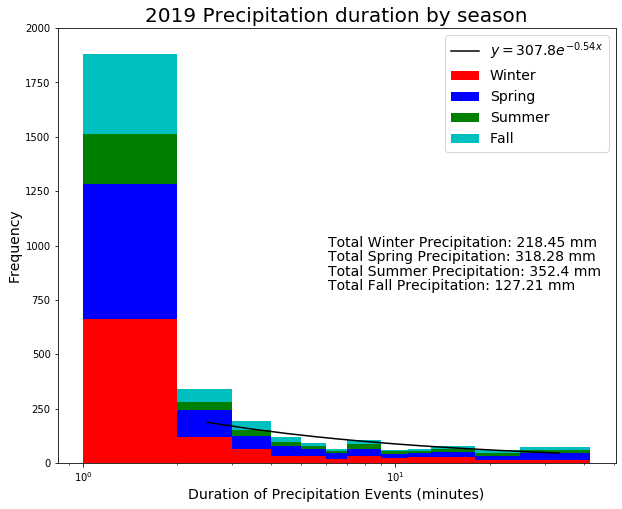
\includegraphics[width=0.675\textwidth]{Figures/More_detail_precip_2019.png}
  \caption[Precipitation histogram for 2019 broken down by
    season]{\label{p2019} Distribution of precipitation duration in
    2019, with a breakdown by seasons. The minimum duration,
    $\tau=1$~min, and the maximum duration over the data set is 368
    min, but the horizontal axis was limited to the 98th percentile of
    the durations, 42~min, for clarity. Superposed is a least-squares
    fit of a line in log-log space of duration versus frequency for
    the entire year, excluding the 1--2~min bin, quoted as the
    equivalent exponential in this space.}
\end{figure}
\begin{figure}[b]
  \centering
  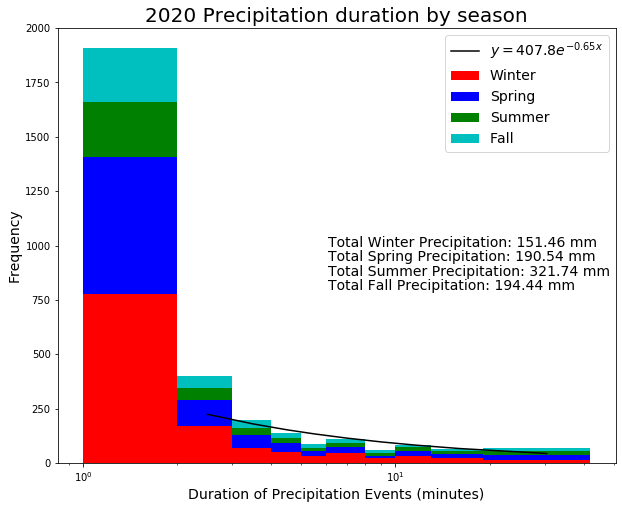
\includegraphics[width=0.675\textwidth]{Figures/precip_2020.png}
  \caption[Precipitation histogram for 2020 broken down by
    season]{\label{p2020} Distribution of precipitation duration
    in 2020, with a breakdown by seasons. 2020 is also
    incomplete as collection still ongoing. The layout is as in
    Figure~\ref{p2019}.}
\end{figure}
\clearpage
\begin{figure}[t]
  \centering
  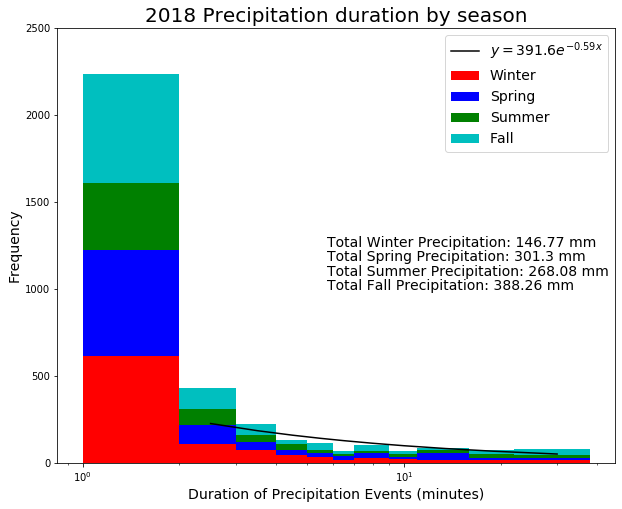
\includegraphics[width=0.675\textwidth]{Figures/precip_2018.png}
  \caption[Precipitation histogram for 2018 broken down by season]{\label{p2018}
    Distribution of precipitation duration in 2018, with a breakdown
    by seasons. The layout is as in Figure~\ref{p2019}.}
\end{figure}

\begin{figure}[b]
  \centering
  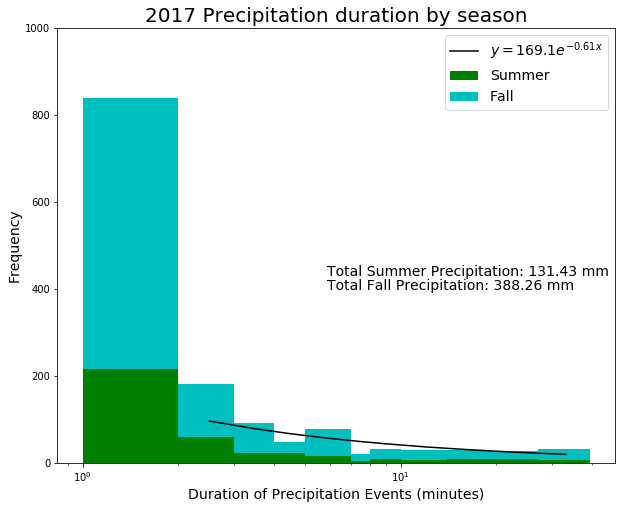
\includegraphics[width=0.675\textwidth]{Figures/precip_2017.png}
  \caption[Precipitation histogram for 2017 broken down by
    season]{\label{p2017} Distribution of precipitation duration in
    2017, with a breakdown by seasons. The layout is as in
    Figure~\ref{p2019}. Note that data collection began on 16 July
    2017.}
\end{figure}
\clearpage

%Is the exponential different for W/S/S/F? Can you tell the difference?
%Is the exponential different for different years? Can you tell the
%difference?  And what summarizes it all. 

\begin{table}[bh]
  \begin{center}
    \begin{tabular}{|l|*{11}{r|}r|}
      \hline
      Season    &       \multicolumn{2}{|c|}{Annual}          & \multicolumn{2}{|c|}{Winter}& \multicolumn{2}{|c|}{Spring}  & \multicolumn{2}{|c|}{Summer} &\multicolumn{2}{|c|}{Fall}  \\
      \hline
      Year      & $\beta $ & $\alpha$  & $\beta $ & $\alpha$ & $\beta $ & $\alpha$ & $\beta $ & $\alpha$ & $\beta $ & $\alpha$\\
      \hline
      2017      & \textit{169}  & \textit{-0.61}  & NaN & NaN & NaN & NaN & \textit{57}  & \textit{-0.70}  & 108  & -0.57  \\
      2018      & 392           & -0.59  & 148 & -0.74 & 125 & -0.76 & 65  & -0.52  & 91 & -0.50  \\
      2019      & 308           & -0.54  & 118  & -0.62 & 107 & -0.58 & 32 & -0.31  & 57 &  -0.60 \\
      2020      & 408           & -0.65   & 201  & -0.80 & 112  & -0.66 & 48  & -0.42 & 64 & -0.66\\
      \hline
    \end{tabular}
  \end{center}
\caption[Year comparison of coefficients of precipitation duration up to its
  98th percentile]{\label{firsttable}Coefficients found from the yearly
  distribution of precipitation duration (as in equation~\ref{expod}) as
  well as the seasonal distribution of precipitation duration. Italics refer
  to values obtained using incomplete information. NaN means there was no
  information. These coefficients were computed using the 0 to 98th
  percentile of precipitation duration.}
\end{table}


 
Based on Table~\ref{firsttable}, the $\beta$ values are similar to
each other with the exception of 2017, which only had partial data
starting in the Summer. Even, with the partial data we have from 2017
and 2020, it is clear that the $\alpha$ values are similar to each
other. Focusing on the years with complete data, 2018 and 2019, it is
clear that yearly variations exists between them. All $\alpha$ values
are negative.

In the seasonal variations, we see that Summer has $\alpha$ values
that are less negative compared to the other seasons as well as having
a lower $\beta$ compared to the other seasons. However looking at
Table~\ref{secondtable}, we see that the summers also have a lot of
precipitation. The fewer amounts of precipitation events in the
Summer, but with a lot of precipitation gives a higher intensity for
the Summer. For the Winter, the $\alpha$ are the furthest from 0 and
the $\beta$ are large. However, Winter tends to have the lowest values
for total precipitation and the combination of lots of preciptation
events and low precipitation totals results in the lowest intensities
among the four seasons.

The Spring appears to mimic the Winter in that there are a lot of
preciptiation events, but also shares the quality of Summer in having
fairly high precipitation totals. The Fall shares the Summer quality
of having relatively few preciptation events, but tends to have
smaller precipitation totals, so its intensity is less than the
Summer, but greater than the winter precipitation intensity.
\begin{table}[t]
  \begin{center}
    \begin{tabular}{|l|*{11}{c|}r|}
      \hline
      Season    &       \multicolumn{2}{|c|}{Annual}          & \multicolumn{2}{|c|}{Winter}& \multicolumn{2}{|c|}{Spring}  & \multicolumn{2}{|c|}{Summer} &\multicolumn{2}{|c|}{Fall}  \\
      \hline
      Year      & T & I  & T & I  & T & I  & T & I  & T & I \\
      \hline
      2017      & \textit{520}  & \textit{0.07}  & NaN & NaN & NaN & NaN & \textit{131}  & \textit{0.07}  & 388  & 0.07  \\
      2018      & 1104           & 0.06  & 147 & 0.03 & 301 & 0.07 & 268  & 0.08  & 388 & 0.07  \\
      2019      & 1016           & 0.06  & 218  & 0.04 & 318 & 0.06 & 352 & 0.11  & 127 &  0.05 \\
      2020      & 858          & 0.06   & 151  & 0.03 & 191  & 0.04 & 322  & 0.12 & 194 & 0.06\\
      \hline
    \end{tabular}
  \end{center}
  \caption[Summary of total precipitation and
    intensity]{\label{secondtable}Total precipitation (in mm) and average
    intensity (in mm/min) of precipitation for each year and season. Italics
    refer to values obtained using incomplete information. NaN means there
    was no information.}
\end{table}
 

Looking at trying to extend the exponential fit towards non-precipitation event durations, the exponentials for such duration, $\delta$ is less negative overall compared to the exponentials from the precipitation event duration, $\alpha$. Some of this is explained from the fact that the duration of non-precipitation events range from 1 minute to over 2000 minutes, whereas the duration of precipitation events range from 1 minute to just over 300 minutes. At the same time how we bin the durations for both precipitation and non-precipitation events will affect how we get the fits. 

\clearpage
\begin{figure}[t]
	\centering
	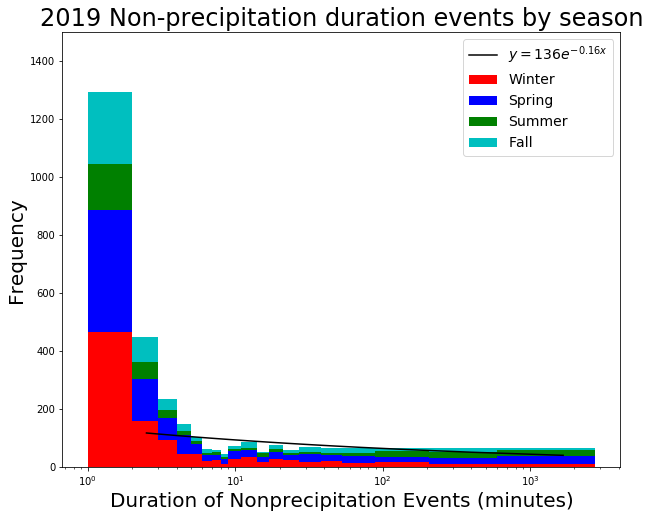
\includegraphics[width=0.675\textwidth]{Figures/nonprecip_2019.png}
	\caption[Histogram of non-precipitation events for 2019 broken
          down by season]{\label{np2019} Distribution of
          non-precipitation event duration in 2019, with a breakdown
          by seasons. The minimum duration, $\tau=1$~min, and the
          maximum duration over the data set is 2613~min, but the
          horizontal axis was limited to the 98th percentile of
          2350~min, for clarity. Superposed is a least-squares fit of
          a line in log-log space of duration versus frequency for the
          entire year, excluding the 1--2~min bin, quoted as the
          equivalent exponential in this space.}
\end{figure}
\begin{figure}[b]
	\centering
	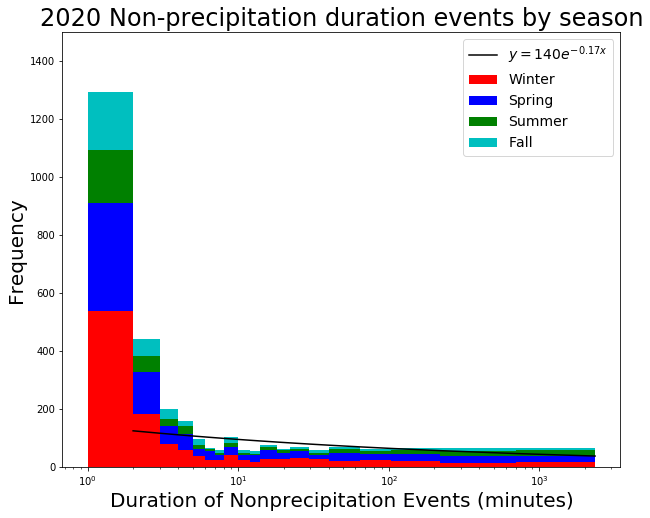
\includegraphics[width=0.675\textwidth]{Figures/nonprecip_2020.png}
	\caption[Histogram of non-precipitation events for 2020 broken down by
	season]{\label{np2020} Distribution of non precipitation event duration
		in 2020, with a breakdown by seasons. 2020 is also
		incomplete as collection still ongoing. The layout is as in
		Figure~\ref{np2019}.}
\end{figure}
\clearpage
\begin{figure}[t]
	\centering
	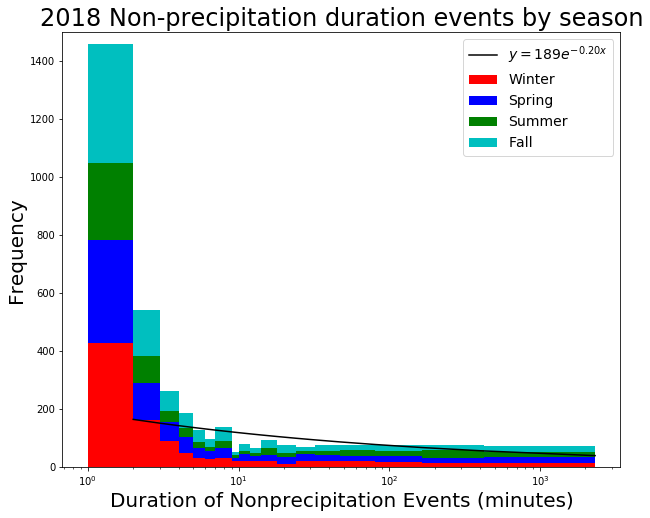
\includegraphics[width=0.675\textwidth]{Figures/nonprecip_2018.png}
	\caption[Histogram of non-precipitation events for 2018 broken down by season]{\label{np2018}
		Distribution of precipitation duration in 2018, with a breakdown
		by seasons. The layout is as in Figure~\ref{np2019}.}
\end{figure}

\begin{figure}[b]
	\centering
	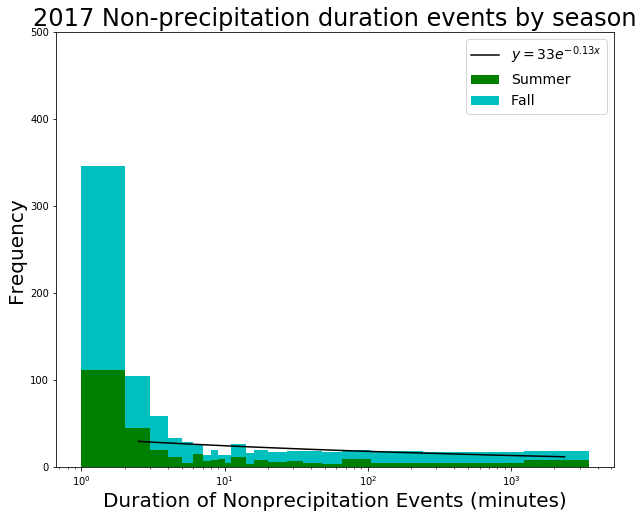
\includegraphics[width=0.675\textwidth]{Figures/nonprecip_2017.png}
	\caption[Histogram of non-precipitation events for 2017 broken down by
	season]{\label{np2017} Distribution of non-precipitation event duration in
		2017, with a breakdown by seasons. The layout is as in
		Figure~\ref{np2019}. Note that data collection began on 16 July
		2017.}
\end{figure}
\clearpage



\clearpage
\begin{figure}[t]
\centering
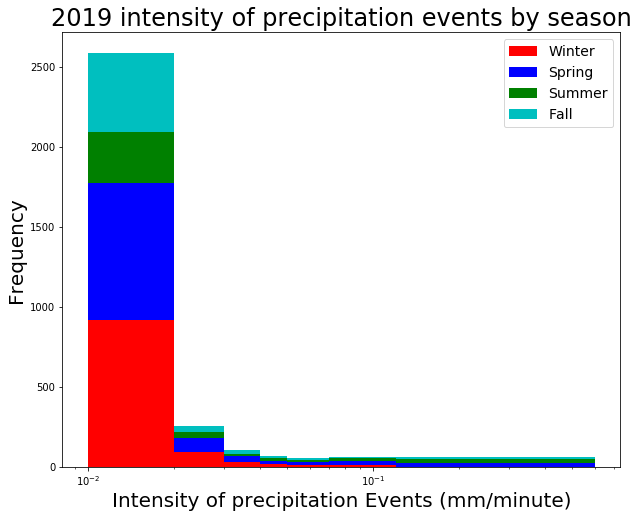
\includegraphics[width=0.675\textwidth]{Figures/inten2019.png}
\caption[Intensity histogram for 2019 broken down by season]
        {\label{i2019}Distribution of precipitation intensity in
          2019, with a breakdown by seasons. The minimum intensity,
          $I=0.01$~mm/min, and the maximum intensity over the data set
          is 0.4~mm/min, but the horizontal axis was limited to the
          98th percentile of the intensity, 0.1~mm/min, for
          clarity. Superposed is a least-squares fit of a line in
          log-log space of duration versus frequency for the entire
          year, %excluding the 0.01~mm/day--0.02~mm/day bin, 
          %quoted as
          %the equivalent exponential in this space.
      }
\end{figure}
\begin{figure}[b]
\centering
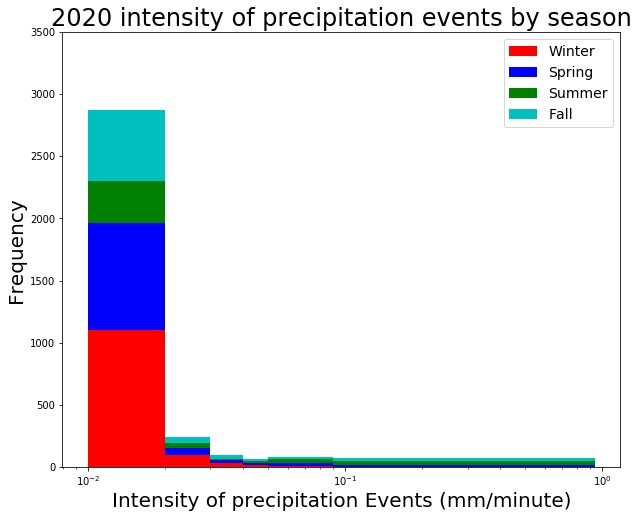
\includegraphics[width=0.675\textwidth]{Figures/inten2020.png}
\caption[Intensity histogram for 2020 broken down by season]
        {\label{i2020}Distribution of precipitation intensity in
          2020, with a breakdown by seasons. 2020 is also incomplete
          as collection still ongoing. The layout is as in
          Figure~\ref{i2019}.}
\end{figure}
\clearpage
\begin{figure}[t]
\centering
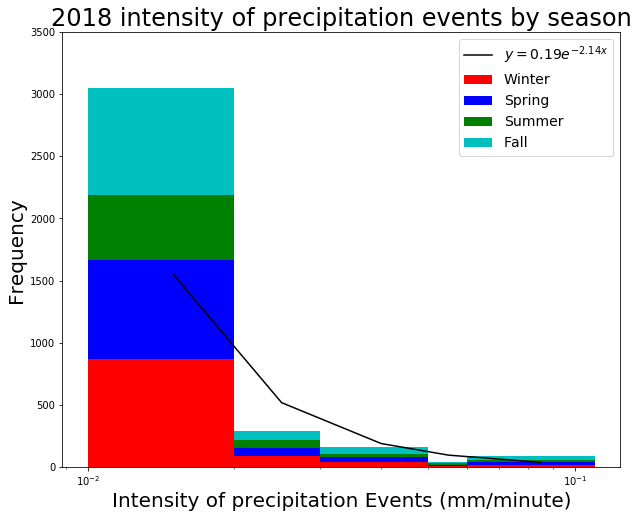
\includegraphics[width=0.675\textwidth]{Figures/inten2018.png}
\caption[Intensity histogram for 2018 broken down by season]
        {\label{i2018}Distribution of precipitation intensity in 2018,
          with a breakdown by seasons. The layout is as in
          Figure~\ref{i2019}.}
\end{figure}

\begin{figure}[b]
\centering
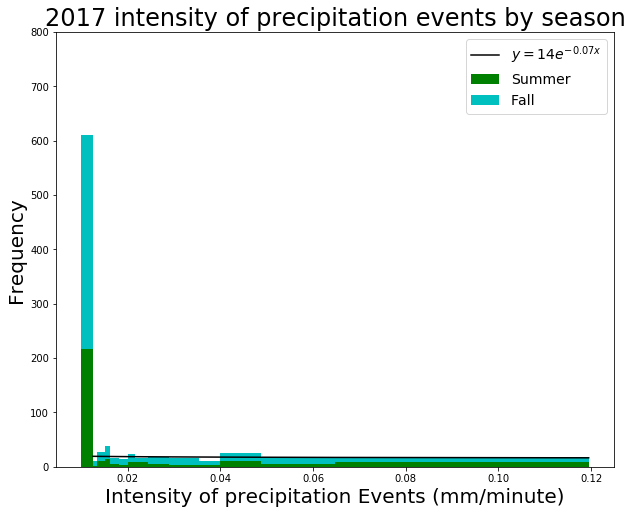
\includegraphics[width=0.675\textwidth]{Figures/inten2017.png}
\caption[Intensity histogram for 2017 broken down by season]
        {\label{i2017}Distribution of precipitation intensity in 2017,
          with a breakdown by seasons. The layout is as in
          Figure~\ref{i2019}. Note that data collection began on 16
          July 2017.}
\end{figure}
\clearpage

\begin{table}[htb]
  \begin{center}
    \begin{tabular}{|l|*{11}{c|}r|}
      \hline Season & \multicolumn{2}{|c|}{Annual} &
      \multicolumn{2}{|c|}{Winter}& \multicolumn{2}{|c|}{Spring} &
      \multicolumn{2}{|c|}{Summer} &\multicolumn{2}{|c|}{Fall} \\ \hline
      Year & $\gamma $ & $\delta$ & $\gamma $ & $\delta$ & $\gamma $ &
      $\delta$ & $\gamma $ & $\delta$ & $\gamma $ & $\delta$\\ \hline 2017 &
      \textit{33} & \textit{-0.13} & NaN & NaN & NaN & NaN & \textit{12} &
      \textit{-0.15} & 19 & -0.12 \\ 2018 & 189 & -0.20 & 59 & -0.28 & 50 &
      -0.29 & 26 & -0.10 & 55 & -0.22 \\ 2019 & 136 & -0.16 & 63 & -0.30 &
      46 & -0.16 & 11 & 0.03 & 24 & -0.16 \\ 2020 & 140 & -0.17 & 64 & -0.23
      & 46 & -0.16 & 13 & -0.02 & 20 & -0.21 \\ \hline
    \end{tabular}
  \end{center}
  \caption[Year comparison of coefficients for non-precipitation events up
    to 98th percentile] {\label{thirdtable_98}Coefficients found from
    the yearly distribution of non-precipitation event duration (as in
    equation~\ref{expod_np}) as well as the seasonal distribution of
    non-precipitation event duration. Italics refer to values obtained using
    incomplete information. NaN means there was no information. Using
    non-precipitation event durations from the 0 to the 98th percentile.}
\end{table}

\begin{table}[htb]
  \begin{center}
    \begin{tabular}{|l|*{11}{c|}r|}
      \hline
      Season    &       \multicolumn{2}{|c|}{Annual}          & \multicolumn{2}{|c|}{Winter}& \multicolumn{2}{|c|}{Spring}  & \multicolumn{2}{|c|}{Summer} &\multicolumn{2}{|c|}{Fall}  \\
      \hline
      Year      & $\epsilon $ & $\zeta$  &  $\epsilon $ & $\zeta$  &  $\epsilon $ & $\zeta$  &  $\epsilon $ & $\zeta$  & $\epsilon $ & $\zeta$ \\
      \hline
      2017      & \textit{0.06}  & \textit{-1.98}  & NaN & NaN & NaN & NaN & \textit{0.03}  & \textit{-1.94}  & 0.04  & -2.00  \\
      2018      & 0.19           & -2.14  & 0.02 & -2.41 & 0.03 & -2.24  & 0.10  & -1.87  & 0.08 & -2.05  \\
      2019      & 0.23           & -2.01  & 0.03 & -2.29 & 0.07 & -2.02 & 0.25 & -1.47 & 0.03 & -2.16  \\
      2020      & 0.06          & -2.38  & 0.002 & -3.00 & 0.02 & -2.38 & 0.10  & -1.74 & 0.02 & -2.18\\
      \hline
    \end{tabular}
  \end{center}
  \caption[Year comparison of coefficients for precipitation
    intensity] {\label{fourthtable}Coefficients found from the yearly
    distribution of precipitation intensity (as in equation~\ref{expod_inten}) as
    well as the seasonal distribution of precipitation
    intensity. Italics refer to values obtained using incomplete
    information. NaN means there was no information. }
\end{table}


In contrast, Table~\ref{fourthtable} for intensity of precipitation events show a more negative exponential compared to either precipitation or non-precipitation event durations. This is partially due to the fact that there are less bins in the intensity of preciptiation events as seen that the vast majority of precipitation events are not particularly intense on average. 




\section{Results\label{sec:results}}
\begin{figure}[t]
	\centering
	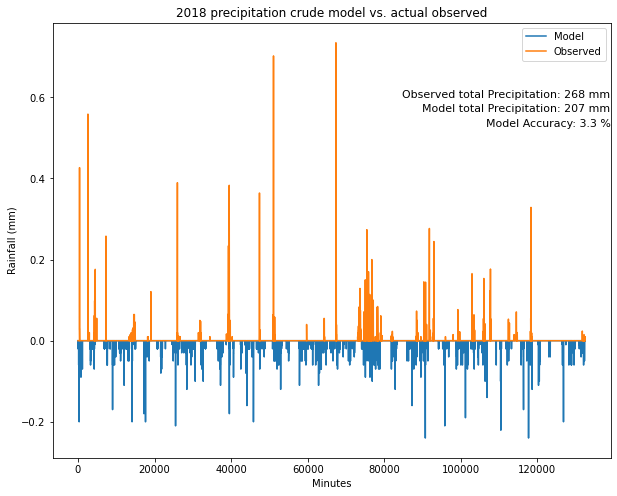
\includegraphics[width=0.75\textwidth]{Figures/better_one_run.png}
	\caption[One run using Summer 2018 climatology]
	{\label{crudemodel}One model run using the exponentials calculated from Summer 2018.  }
\end{figure}
Running the model one hundred times let us look at what the average precipitation total the model yields, it yields 195 mm compared to the Summer 2018 total of 268 mm that we used. Furthermore, the accuracy of model precipitation matching model precipitation is only 6$\%$. Looking at \ref{crudemodel}, we see that the model precipitation total is lower than the actual precipitation observed in the Summer of 2018. Furthermore, the precipitation seem to be more frequent compared to the observed 2018 Summer data. 


\section{Discussion\label{sec:discussion}}
This section is blank for now. 

\section{Conclusions\label{sec:conclusions}}
This section is blank for now. 

%--References
\small
\renewcommand{\bibsep}{0em}

\renewcommand{\bibname}{References}
\bibliographystyle{Latex/gji}
\bibliography{refs}

\end{document}
